% =====================================================================
% NOTE TO AUTHOR (read before compiling):
%   September 15, 2026 revision draft based on the rejected BlackboxNLP 2026
%   submission; no future venue has been selected. Drop THIS file
%   (acl_latex.tex) and custom.bib into the official ACL Overleaf template
%   (ships acl.sty + acl_natbib.bst), then compile with pdfLaTeX + BibTeX.
%   The draft remains in [review] mode with an anonymous author block.
%
%   DATA: stagewise, targeted-control, and corpus numbers come from
%   out/results/summary_v3.json (plus-one-corrected run, 5 canonical seeds,
%   4 extension seeds, 140 prompts) and matched_control_stagewise.json;
%   audit numbers come from ai_consensus_validation_v3.json. Derived stats via experiments/monte_carlo_correction.py,
%   derive_paper_stats.py, between_condition_stats.py, stage_condition_gaps.py,
%   multiple_testing.py, threshold_robustness.py, audit_cluster_bootstrap.py,
%   dpo_pairwise.py, dpo_phrase_robustness.py, and raw_output_robustness.py.
%   Primary inference = prompt-clustered permutation tests (in the artifact).
%   COMPLETED DIAGNOSTIC: two independent blinded AI passes over 120 sentences,
%   with three disagreements adjudicated by Claude Opus 4.8. This is explicitly
%   AI-only and is not human validation. The exploratory paired DPO conditional
%   fit was completed under its dated protocol. PENDING: causal leave-cluster-out,
%   Stage-2 Dolmino index, and independent human validation. No prospective experiment or human-label result
%   is represented as complete in this draft.
% =====================================================================

\documentclass[11pt]{article}

\usepackage[review]{acl}

\usepackage{times}
\usepackage{latexsym}
\usepackage[T1]{fontenc}
\usepackage[utf8]{inputenc}
\usepackage{microtype}
\usepackage{booktabs}
\usepackage{graphicx}
\usepackage{amsmath}

% Absorb small overfulls from long \texttt{} identifiers.
\emergencystretch=3em

\title{Measuring Advice-Style Language in OLMo-2:\\
Effects of Detection Rules and Response Length}

% === Anonymous author block for review (current) ===
\author{Anonymous Submission}

\begin{document}
\maketitle

\begin{abstract}
Phrase counts can make model responses auditable, but they also rise when
answers are longer or a detector accepts loose semantic matches. We ask how
detection rules and response length affect conclusions about advice-style
language across OLMo-2 post-training. We analyze a five-condition, 140-prompt
battery at public 1B and 7B checkpoints, audit the historical detector against
120 AI-labeled sentences, and search about 378,000 DPO pairs per model. The
combined detector has low precision against these narrow AI targets; human
validation remains pending. In the recovered final-7B cache, the empathy-opener
advice-minus-emotional-control point estimate changes from $-.147$ on full
responses to $+.253$ at 64 tokens; the full-response estimate is uncertain.
Across same-interface SFT-to-DPO checkpoints, validation-marker gaps increase
while structuring-marker gaps contract. In exploratory paired DPO models that
flexibly condition on response length, broad referral/disclaimer and
structuring phrases remain positively associated with the chosen side, while
narrower-referral intervals include one. These are detector-defined
comparisons, not estimates of semantic empathy or causal training effects.
\end{abstract}

\section{Introduction}

Suppose a model answers ``I've been feeling anxious and cannot sleep---what
should I do?'' with ``That sounds really difficult. Here are a few steps you
can try.'' The historical rules count both an empathy-opener and a structuring
marker. Now consider the constructed fragment ``A checklist may help. That
sounds really useful for packing.'' It also triggers the empathy-opener rule:
the phrase \emph{that sounds really} appears in the second sentence, even though
it appraises a checklist rather than a person's emotion. This is an illustration
of rule behavior, not a sampled output or validation example.

Such cases matter beyond one imperfect detector. Checkpoint and condition
comparisons often reduce free-form answers to occurrence rates. A longer answer
offers more phrases and sentences to search, and an embedding rule can add
matches that an exact rule would reject. A change in occurrence rate can
therefore reflect the model response, the amount of text observed, the matching
rule, or all three. Without separating them, an apparent behavioral trajectory
may instead be a measurement trajectory.

This paper asks one question: \emph{How do detection rules and response length
change conclusions about advice-style language across OLMo-2 post-training?}
A \textbf{marker} is a specified textual feature, such as one of the phrases in
our lexicon. A \textbf{detector} is the algorithm that decides whether a marker
category occurs. A detector output becomes a \textbf{proxy} when it stands in
for a broader construct such as empathy. In particular, the category named
\emph{empathy-opener} in the original artifact is searched anywhere in an
answer, and \emph{referral/disclaimer} combines referrals, disclaimers, and
professional-language mentions. Neither output is a semantic judgment.

OLMo-2 is useful for this measurement study because its final Instruct model is
the product of four public data-bearing stages:
pretraining, supervised fine-tuning (SFT), direct preference optimization
(DPO), and reinforcement learning with verifiable rewards (RLVR)
\citep{olmo2025olmo2}. OLMo-2 offers an unusually complete public chain of
post-training data and intermediate checkpoints.

\newpage
\paragraph{Findings and contributions.}
\begin{enumerate}\itemsep2pt
\item In the recovered final-7B responses, component and output-window choices
change targeted-control contrasts; an AI-label diagnostic traces every sampled
union false positive to the embedding component. Human validation is pending.
\item Under the historical detector, same-interface SFT-to-DPO validation gaps
increase at both model sizes while structuring gaps contract. Base-to-SFT
comparisons remain confounded with prompt serialization.
\item In exploratory paired DPO models, broad referral/disclaimer and
structuring associations remain positive after flexible length conditioning;
both narrower-referral intervals include one.
\end{enumerate}

\section{Related Work}

\paragraph{Behavioral tests and construct validity.}
Our targeted prompt battery follows the behavioral-testing principle that
targeted capabilities require controlled tests beyond aggregate accuracy
\citep{ribeiro2020checklist}. Pythia makes dense public checkpoints available
for training-dynamics research \citep{biderman2023pythia}; checkpoint studies
have tracked how loss and downstream behavior change during pretraining
\citep{xia2023trajectories}. We instead compare named post-training stages and
test changes in condition gaps rather than raw behavior rates.

Very recent work traces situation modeling and putative mentalizing across
OLMo-2 and Pythia stages while stress-testing construct validity
\citep{riviere2026developmental}. It is closest in model family and
developmental framing; its caution about mapping task outputs to cognitive
constructs directly motivates our proxy terminology. Emotional-support work
typically grounds support strategies in theory and human annotation
\citep{liu2021emotional}, while empathy research warns that incompatible
operational definitions undermine comparison \citep{lahnala2022critical}.
Recent studies compare human and LLM judgments directly
\citep{welivita2026empathetic}; in mental-health settings, LLM judges are less
reliable for affective properties such as empathy \citep{badawi2026trust}.
Accordingly, our AI-only audit diagnoses a rule rather than validating a human
construct.

\paragraph{Length in preference evaluation.}
Preference and reward-model data can encode length correlations
\citep{singhal2023long}, and length-controlled evaluation can change model
rankings \citep{dubois2024length}. Our contribution is narrower: we test how
response length changes marker-specific exact-match differences in the OLMo-2
DPO mixtures. We report the post-hoc length strata alongside an exploratory
paired conditional model whose protocol was written before its new fits, after
the aggregate results were known. Both describe associations rather than a
causal adjustment.

\paragraph{Open models, data, and the attribution boundary.}
Tulu-3 \citep{lambert2024tulu3} is the recipe behind OLMo-2's post-training;
the SFT mixtures, DPO preference mixes, and RLVR sets are public, as is oasst1
\citep{kopf2023oasst1} (itself an internal subset of the Tulu-3 mixtures).
Public post-training data and checkpoints make detector trajectories and corpus
co-occurrences auditable. Exact-substring tools such as infini-gram
\citep{liu2024infinigram} and output-to-pretraining tracing in OLMoTrace
\citep{liu2025olmotrace} motivate the supporting corpus search. They do not
turn co-occurrence into attribution. LIMA \citep{zhou2023lima} and
\citet{ghosh2024closer} debate whether alignment surfaces latent style from a
small number of demonstrations; our weak marker correlations cannot resolve
that broader hypothesis.

LESS uses optimizer-aware gradient similarity to select influential instruction
data \citep{xia2024less}; \citet{xiao2026probe} perform probe-based causal
attribution on OLMo-2 DPO and mitigate a behavior by editing top-attributed
preference pairs. Our evidence is observational: it identifies detector changes
and phrase co-occurrence across public stages, but does not establish which
examples caused an output.

\section{Measurement and Study Design}

\subsection{Operational categories and fixed detector}
\label{sec:method-detect}
A hand-seeded, inspectable lexicon specifies four marker categories using the
artifact's historical names: \emph{empathy-opener}, \emph{validation-phrase},
\emph{referral/disclaimer} (artifact key \texttt{disclaimer}), and
\emph{structuring-marker} (\texttt{structure}). The names label rules rather
than validated constructs. The empathy-opener rule searches every sentence, not
only an opening span. Referral/disclaimer is a broad combined rule that also
includes professional-language fragments such as ``consult a'' and ``medical
professional''; it is not a detector of referrals alone. A fifth historical
category, \texttt{crisis\_referral}, is excluded from the four-category analysis
after producing 0 true positives and 11 false positives in the audit.

The historical comparisons use archived detector outputs and the original
primary threshold rather than rules selected for the present revision. The detector
takes the union of case-insensitive substring matching and an e5-small embedding rule
\citep{wang2024e5}: a response is positive when either an exact phrase appears
or any sentence reaches cosine similarity $\tau=0.82$ to a category exemplar.
We also examine $\tau=0.80$ and $0.84$. Longer responses supply more sentences
and therefore more opportunities for the embedding rule to fire. The complete
specification used to reproduce the July final-7B response analysis is in
Appendix~\ref{app:lexicon}; the raw-cache diagnostics preserve that version
rather than retrospectively improving it. Archived stage summaries are analyzed
as historical outputs. Because most stagewise raw responses are unavailable, we
do not claim to have re-executed every stage under a byte-identical detector.

\paragraph{Construction and pilot overlap.} The accompanying pilot file contains eight
personal-advice prompts and four general-facts controls used while hand-seeding the proxy; all
12 reappear in the 140-prompt battery. We therefore do not call the full battery
held out. A final-7B sensitivity excluding those 12 leaves the advice--factual
gaps similar (Appendix~\ref{app:response-robustness}). The sample sizes refer to
distinct datasets: the 140 prompts form the marker evaluation, whereas 120 stratified final-model
sentences form an AI-label diagnostic. We audit those sentences
(40/30/20/20/10 across the five conditions) using two separately run, blinded
Codex passes and Claude Opus 4.8 adjudication of their three disagreements.
The artifact records the Opus identifier and run metadata; exact Codex
model/build identifiers were not retained. This is an AI diagnostic, not human
validation. The revision materials include the labels, adjudication
reasons, and detector (Section~\ref{sec:detval};
Appendix~\ref{app:lexicon}).

\subsection{Prompt conditions and generation}
\label{sec:method-battery}
Five conditions target different aspects of advice-style responses:
\emph{personal advice} (60 personal or emotional help requests), \emph{general
facts} (30 knowledge questions), \emph{emotion without a request} (20 prompts
about emotional topics without asking for help), \emph{neutral how-to} (20
requests for practical advice without emotional stakes), and \emph{health
facts} (10 impersonal clinical-information questions). These controls separate
request type, emotional content, and domain. They target conceptual axes but are
not paired counterfactuals or topic-matched scenarios; non-significance is not
interpreted as equivalence. The final-model battery and the canonical
personal-advice/general-facts checkpoint trajectories use five sampled generations
per prompt (temperature $0.7$, top-$p$ $0.9$, 256 new tokens, distinct seeds).
The Base/SFT/DPO five-condition extension uses four; its
balanced comparisons use seeds 0--3 for every condition.

Table~\ref{tab:study-map} separates the study's evidence sources. The final
condition battery asks whether a marker is specific to personal advice. The
checkpoint grid asks when advice-minus-general-facts gaps change. The AI-label
diagnostic asks how the detector relates to narrow sentence labels. The DPO
analysis asks whether exact phrases differ between chosen and rejected answers,
and how those differences relate to response length.

\begin{table*}[t]
\centering
\small
\setlength{\tabcolsep}{4pt}
\begin{tabular}{p{2.4cm}p{3.5cm}p{4.7cm}p{4.1cm}}
\toprule
Analysis & Material & Comparison & Main scope limit \\
\midrule
Final conditions & 140 prompts, five conditions, five generations & Personal advice versus general facts, emotion without a request, neutral how-to, and health facts & Author-written controls are not topic-paired counterfactuals \\
Checkpoint grid & 90 personal-advice/general-facts prompts, five generations & Changes in the advice-minus-facts gap across public 1B and 7B stages & Base-to-SFT also changes prompt serialization; most raw responses are unavailable \\
AI-label diagnostic & 120 sentences from 97 final responses & Historical detector versus narrow AI consensus labels & No human labels; referral target is narrower than the detector \\
DPO pairs & 378,301 1B and 378,341 7B pairs & Exact chosen-versus-rejected matches, with paired flexible length conditioning & Observational; conditioning changes the estimand; mixtures share 21,508 pairs \\
\bottomrule
\end{tabular}
\caption{Evidence map. Each analysis answers a different part of the measurement
question and has a different unit and scope limit.}
\label{tab:study-map}
\end{table*}

\subsection{Inference at the prompt level}
\label{sec:method-stats}
The clustering unit is the prompt: each prompt contributes its mean
detector-positive indicator over its four or five generations, and condition rates are means over
prompts. All between-condition inference uses prompt-clustered permutation
tests (10{,}000 permutations of prompt-level means; two-sided;
Monte Carlo $p=(b+1)/(B+1)$). Benjamini--Hochberg correction is applied
separately to the 24 final-condition contrasts, 28 advice/general-facts adjacent-stage
interactions, 24 targeted-control stage interactions, and 8 historical DPO pairwise tests.
We do \emph{not} treat generations as independent Bernoulli trials:
all condition and stage tests operate on prompt-level generation means.

\subsection{Exploratory paired DPO length model}
\label{sec:method-dpo-conditional}
For each of three exact marker groups and each model size, the new paired model
uses the conditional likelihood $\sum_i\log\sigma[\boldsymbol\beta^\top
(\mathbf{x}_{ic}-\mathbf{x}_{ir})]$ with no intercept. The features are the
chosen-minus-rejected marker flag and differences in a restricted cubic spline
of $\log(1+\text{words})$. Five pooled knots were fixed at the 5th, 27.5th,
50th, 72.5th, and 95th percentiles (7, 78, 204, 374, and 739 words) before
fitting. Intervals use a prompt-cluster sandwich covariance with finite-cluster
correction. The resulting conditional odds ratio (OR) equals one when the model
estimates no marker--choice association at the modeled lengths; it is not a
percentage-point change in choice probability. Conditioning on an observed
response property changes the estimand and does not remove bias or identify a
causal effect. The six fits are exploratory, not preregistered or confirmatory;
Benjamini--Hochberg values across them are secondary summaries.

\subsection{Checkpoint evaluation}
\label{sec:method-stagewise}
The same evaluation runs on every public checkpoint: 1B
Base$\to$SFT$\to$DPO$\to$RLVR1$\to$Instruct; 7B
Base$\to$SFT$\to$DPO$\to$Instruct. Base checkpoints have no chat template and
use a plain Question/Answer format, whereas post-trained checkpoints use their
official chat template. Thus Base$\to$SFT is a stage-plus-interface
transition and cannot isolate SFT training. No serialization crossover was run;
we demote that transition throughout. The
stagewise grid runs the 90 personal-advice plus general-facts prompts at every checkpoint. All five
conditions run on the final models and, in the four-seed specificity extension,
at Base, SFT, and DPO.

Corpus searches provide secondary context. For each stage's available indexed data
we search the exact Stage-1 corpus
(\texttt{v4\_olmo-mix-1124\_llama}; novelty $=1-$verbatim coverage), each
model's exact SFT mixture (\texttt{tulu-3-sft-olmo-2-mixture-0225} for 1B;
\texttt{tulu-3-sft-olmo-2-mixture} for 7B) in DuckDB with assistant-only scoping
(866{,}138 conversations for 1B and 939{,}344 for 7B; oasst1 is not searched
separately since it is an internal subset), the DPO preference mixes
(pair-level chosen-only/rejected-only counts, exact McNemar tests, and phrase
occurrences per million response words), and the
RLVR sets. SFT recoverability compares seeded marker phrases against
length-matched topical controls from the same answers, per-million documents,
with a distinct-phrase leave-one-out. Stage-2 mid-training uses
Dolmino-Mix-1124, for which no public index was available; the corpus trace is
therefore incomplete.

\paragraph{Reproducibility.} Stagewise, condition, and corpus numbers derive
from \texttt{summary\_v3.json} and accompanying scripts under
\texttt{experiments/}. The revision materials include prompts, the lexicon,
seeds, thresholds, and adjusted-$p$ output. Audit numbers are materialized in
\texttt{ai\_consensus\_validation\_v3.json}, which also contains both 120-item
passes, consensus labels, Opus decisions, and reasons.
The paired DPO features, parity manifest, conditional estimates, and dated
exploratory protocol are stored under
\texttt{output/revision/dpo\_conditional/} and \texttt{out/paper/}.

\section{Results}
\label{sec:results}

We first audit the measurement rule, then report condition and checkpoint
comparisons under that rule, and finally examine the association between DPO
phrase differences and response length. This order matters because the audit
limits what the subsequent detector-positive rates can mean.

\subsection{AI-label diagnostic and rule sensitivity}
\label{sec:detval}

A condition-stratified random audit samples 120 final-model sentences across
all five conditions (40 personal advice, 30 general facts, 20 emotion without a
request, 20 neutral how-to, and 10 health facts). The sample contains 56 sentences from the 1B
model and 64 from the 7B model, drawn from 97 distinct seed-0 responses. It was
not stratified on detector predictions, and multiple sentences can come from
one response. Two independent blinded Codex passes agree exactly on 117 of 120
sentences (97.5\%). Category agreement is 99.2--100\%; Cohen's $\kappa$ is
.885 for empathy expression, .663 for validation, 1.000 for referral, and .978
for structuring. Claude Opus 4.8 adjudicates the three disagreements. These are
AI-consensus labels under specific prompts and models, not human ground truth.

Against that consensus, the union detector has low precision and
category-dependent recall (Table~\ref{tab:detval}). The audit's referral label
is narrower than the detector: it requires an actual recommendation to seek a
qualified professional, while the historical referral/disclaimer rule also
matches disclaimers and professional-language mentions. Its 0.06 precision
therefore reflects both broad detector behavior and target misalignment; it
should not be read as the accuracy of a pure referral detector. Empathy and
validation recall are each 0.50. Errors vary by condition, so subtracting
condition rates does not guarantee cancellation. The detector overpredicts
positives in this sample, although the rates are not formal upper bounds because
recall is below one.

Exact substring matching has no false positives in these 120 sentences but
misses many AI-labeled positives. Its true-positive/false-positive/false-negative
counts are 2/0/2 for empathy expression, 1/0/1 for validation, 1/0/0 for
referral, and 9/0/21 for structuring. Every union false positive is introduced
by the embedding component. The union raises structuring recall from 0.30 to
0.87, with lower precision. Component choice is therefore part of the
measurement question.

The recovered 700-response cache permits a separate response-level diagnostic
for the final 7B checkpoint only. Advice responses average 244 tokens and
factual responses 187; the three targeted-control means are 251--255 tokens.
For the category historically called empathy-opener, the recovered union rates
on full responses are $.6133$ for advice and $.7600$ for emotion without a
request (difference $-.1467$, $p=.08839$). At 64 tokens they are $.3833$ and
$.1300$ (difference $+.2533$, $p=.00340$); at 128 tokens they are $.4933$ and
$.4300$ (difference $+.0633$, $p=.48845$). Thus the point estimate changes sign
at 64 tokens, while the full-response and 128-token comparisons are uncertain.
Validation remains positive, moving
from $.250$ to $.177$; referral/disclaimer moves from $.090$ to $.113$; and
structuring remains near zero, moving from $-.030$ to $-.033$. On full
responses, exact-only advice-minus-targeted-control contrasts are $.323$ for
empathy, $.153$ for validation, $.157$ for referral/disclaimer, and $.390$ for
structuring. One recovered health-facts response illustrates the opportunity
mechanism: ``Here are some key points based on research findings'' occurs after
the first 64 tokens, so the exact structuring rule fires on the full answer but
not on its 64-token prefix. This is a detector example, not a judgment about the
answer's quality. These component and window checks qualify the final-7B result; raw
responses are unavailable for the other checkpoints, so they do not validate
the stagewise trajectories.

\begin{table}[t]
\centering
\small
\begin{tabular}{lcccc}
\toprule
category & P & R & F1 & tp/fp/fn \\
\midrule
empathy expr. & 0.22 & 0.50 & 0.31 & 2/7/2 \\
validation & 0.33 & 0.50 & 0.40 & 1/2/1 \\
ref./discl. & 0.06 & 1.00 & 0.12 & 1/15/0 \\
structuring & 0.49 & 0.87 & 0.63 & 26/27/4 \\
\bottomrule
\end{tabular}
\caption{Union-detector precision, recall, and F1 against the adjudicated
120-sentence AI consensus ($\tau=0.82$). This is a diagnostic against an AI
annotation construct, not human validation. The referral annotation is narrower
than the combined historical referral/disclaimer rule. Response-cluster
bootstrap intervals appear in Appendix~\ref{app:audit-bootstrap}.}
\label{tab:detval}
\end{table}

\subsection{Controls change the apparent category profile}
\label{sec:decomposition}

Table~\ref{tab:conditions} gives mean prompt-level proxy-positive rates per condition on
the final models; Table~\ref{tab:contrasts} tests advice against each targeted
control. Against general-facts controls every category separates sharply in both
models (all prompt-clustered $p\leq.0002$). For referral/disclaimer, the 1B
model has rates .900 on personal advice and .080 on general-facts prompts; the 7B model has
rates .913 and .060.

Targeted controls change the interpretation. At $\tau=.82$, the category
historically called empathy-opener fires more often when emotion is present without an advice request than
advice: .790 versus .590 for 1B ($p=.010$), and .760 versus .617 for 7B
($p=.098$). These are archived summary values. In the separately reconstructed
final-7B cache, the corresponding full-response advice rate is $.6133$
($p=.08839$ for the $-.1467$ gap), and the point estimate changes sign at 64
tokens as reported above. Structuring is high on both advice forms: the personal-minus-
neutral-how-to difference is .000 for 1B ($p=1.0$) and $-.030$ for 7B
($p=.574$). These are tests for a difference, not equivalence tests.

The broad referral/disclaimer category is also common outside personal advice.
It fires on .740 of neutral-advice prompts for 1B and .720 for 7B, and on .820
of health-facts prompts for both models. Its advice-minus-health-facts
difference is small and not significant: .080 for 1B ($p=.352$) and .093 for
7B ($p=.159$). The validation-phrase union output is higher on advice than every
targeted control for both models (all unadjusted $p\leq.0044$; all BH-adjusted
$q\leq.0082$). These marginal profiles differ, but weak correlations do not
establish the absence of a latent response template. The comparisons are
detector-dependent, and the small, mixed 1B--7B differences do not support a
scaling claim.

\begin{table*}[t]
\centering
\small
\setlength{\tabcolsep}{5pt}
\begin{tabular}{llrrrrr}
\toprule
Marker output & Model & Personal advice & General facts & Emotion, no request & Neutral how-to & Health facts \\
\midrule
empathy opener  & 1B & 0.590 & 0.040 & \textbf{0.790} & 0.020 & 0.340 \\
                & 7B & 0.617 & 0.027 & \textbf{0.760} & 0.070 & 0.360 \\
validation phr. & 1B & 0.363 & 0.007 & 0.120 & 0.000 & 0.040 \\
                & 7B & 0.383 & 0.013 & 0.130 & 0.030 & 0.060 \\
ref./discl.     & 1B & 0.900 & 0.080 & 0.510 & 0.740 & 0.820 \\
                & 7B & 0.913 & 0.060 & 0.540 & 0.720 & 0.820 \\
structuring     & 1B & 1.000 & 0.580 & 0.820 & \textbf{1.000} & 0.920 \\
                & 7B & 0.970 & 0.547 & 0.830 & \textbf{1.000} & 0.840 \\
\bottomrule
\end{tabular}
\caption{Mean prompt-level union-detector rate per condition (final models, $\tau=0.82$;
each prompt averaged over 5 generations). Bold marks the cells that break the
``advice-specific'' reading: the empathy-opener output peaks when emotion appears
without an advice request, and structuring is at ceiling on neutral how-to prompts. The
audit shows overprediction in its sentence sample but does not recalibrate these
response-level rates (Section~\ref{sec:detval}); \texttt{crisis\_referral} is
excluded (0 TP / 11 FP in the 120-sentence audit).}
\label{tab:conditions}
\end{table*}

\begin{table}[t]
\centering
\small
\setlength{\tabcolsep}{2pt}
\begin{tabular}{@{}llrrr@{}}
\toprule
Marker & Model & \shortstack{Emotion,\\no request} &
\shortstack{Neutral\\how-to} & \shortstack{Health\\facts} \\
\midrule
empathy    & 1B & $-.200$ (.010) & $.570$ (.0002) & $.250$ (.016) \\
           & 7B & $-.143$ (.098) & $.547$ (.0002) & $.257$ (.031) \\
validation & 1B & $.243$ (.003)  & $.363$ (.0002) & $.323$ (.003) \\
           & 7B & $.253$ (.003)  & $.353$ (.0003) & $.323$ (.004) \\
referral   & 1B & $.390$ (.0002) & $.160$ (.006) & $.080$ (.352) \\
           & 7B & $.373$ (.0002) & $.193$ (.001) & $.093$ (.159) \\
structuring & 1B & $.180$ (.0002) & $.000$ (1.0) & $.080$ (.018) \\
           & 7B & $.140$ (.004) & $-.030$ (.574) & $.130$ (.026) \\
\bottomrule
\end{tabular}
\caption{Each cell is personal advice minus the named targeted control
(prompt-clustered permutation $p$, 10k draws). Benjamini--Hochberg correction
across the 24 displayed tests leaves
the validation-phrase result unchanged (all $q\leq.0082$). Non-significant
cells mean ``no detected difference,'' not equivalence.}
\label{tab:contrasts}
\end{table}

\paragraph{Marker co-occurrence.}
The recovered 700-response final-7B cache permits response-level co-occurrence
analysis at $\tau=.82$. Among advice responses, 4.7\% contain one proxy, 29.0\%
two, 40.7\% three, and 25.7\% all four (none contain zero). Referral/disclaimer
is present in 93.0\% of validation-positive advice responses, while pairwise phi
correlations range from $-.14$ to $.21$. The categories often co-occur, but
these weak correlations alone neither establish nor rule out a latent response
template. The accompanying materials include condition-level joint
distributions and all pairwise correlations
(Appendix~\ref{app:response-robustness}).

\subsection{Checkpoint gaps change by marker}
\label{sec:stagewise}

Raw advice-side rates rising across stages would be ambiguous because post-training
could simply make \emph{all} outputs more cautious and listy. A more informative
operational quantity is the personal-advice-minus-general-facts gap $\Delta_s$ at each stage
(Table~\ref{tab:stagewise}) and its \emph{change} across adjacent stages, a
stage$\times$condition difference-in-differences tested with a prompt-clustered
permutation test on per-prompt stage trajectories (Table~\ref{tab:interaction};
10k permutations, with 60 personal-advice prompts and 30 general-facts prompts).

All eight Base-to-SFT/interface changes are positive and six survive BH
correction. For referral/disclaimer, the change is +.253 for the 1B model and
+.243 for the 7B model; for structuring it is +.337 and +.227, respectively.
Validation does not survive correction ($q=.137$ for 1B and $q=.121$ for 7B).
Every category is already detector-positive at Base. Because Base uses plain QA
and SFT uses the chat template, these changes cannot isolate training from
serialization.

The same-interface SFT-to-DPO transition differs by category. The validation
gap increases by +.213 for 1B ($q=.002$) and +.147 for 7B ($q=.021$). The 1B
referral/disclaimer gap increases by +.190 ($q=.002$), while its 7B change of
+.083 is not significant after correction ($q=.203$). The empathy-opener
changes are also not significant after correction. The structuring gap
contracts by $-.367$ for 1B and $-.277$ for 7B (both $q=.002$), because DPO
raises detector-positive structuring on factual answers while advice-side rates
are near ceiling. Preference-data co-occurrence cannot independently explain
these trajectories: length-stratified estimates differ sharply, while the
exploratory conditional models retain smaller broad-referral and structuring
associations (Table~\ref{tab:dpo}).

No RLVR or final-merge gap change is significant (all raw $p\geq.168$). These
tests describe the outputs of the fixed detector. Because the audit finds
condition-dependent false positives and does not span checkpoints, they do not
by themselves establish changes in human-judged behavior prevalence.

\begin{table}[t]
\centering
\small
\setlength{\tabcolsep}{1.5pt}
\begin{tabular}{@{}llrr@{}}
\toprule
Model & Marker & \shortstack{Base$\to$SFT\\+ interface} &
SFT$\to$DPO \\
\midrule
1B & empathy opener & $+0.190$ (.004) & $+0.117$ (.121) \\
1B & validation phrase & $+0.093$ (.137) & $+0.213$ (.002) \\
1B & referral/disclaimer & $+0.253$ (.002) & $+0.190$ (.002) \\
1B & structuring & $+0.337$ (.002) & $-0.367$ (.002) \\
\midrule
7B & empathy opener & $+0.263$ (.002) & $+0.070$ (.387) \\
7B & validation phrase & $+0.103$ (.121) & $+0.147$ (.021) \\
7B & referral/disclaimer & $+0.243$ (.002) & $+0.083$ (.203) \\
7B & structuring & $+0.227$ (.002) & $-0.277$ (.002) \\
\bottomrule
\end{tabular}
\caption{Change in the personal-advice-minus-general-facts detector gap across transitions
(plus-one-corrected prompt-clustered permutation tests, 10k draws; displayed
$q$ is BH-adjusted across all 28 adjacent-stage$\times$proxy tests). The
Base$\to$SFT column also changes the input serialization and is not a clean SFT
effect. Later raw $p\geq.168$.}
\label{tab:interaction}
\end{table}

\paragraph{Comparisons with targeted controls.} The four-seed
Base/SFT/DPO extension tests 24 planned stage$\times$control interactions
(Appendix~\ref{app:matched-stage}). Four survive BH correction at $\tau=.82$.
For empathy relative to emotion without an advice request, the 7B Base$\to$SFT/interface
transition increases the advice gap
($+0.358$, $q=.016$), but DPO reverses it at both 1B ($-0.467$, $q=.001$) and
7B ($-0.642$, $q=.001$). At 7B, SFT also shifts structuring toward neutral
advice ($-0.208$, $q=.026$). No validation or referral interaction survives
$q<.05$; 1B DPO validation tendencies have $q=.059$--$.095$. The threshold
sweep yields three significant interactions at $\tau=.80$, four at $.82$, and
five at $.84$; only the two 7B
empathy transitions survive at all three thresholds. Thus the broad
advice-minus-general-facts changes cannot all be read as advice-specific.

\subsection{DPO phrase differences track response length}
\label{sec:datalayers}

The exact mixtures contain 378{,}301 preference pairs for 1B and 378{,}341 for
7B. Chosen responses are slightly shorter in aggregate, yet exact
referral/disclaimer and structuring matches favor the chosen side (Table
\ref{tab:dpo}). Only 19.1\% and 18.7\% of pairs fall within $\pm20$ words. In
that post-hoc stratum, broad-referral differences are near zero and structuring
differences remain positive but much smaller; outside it, differences follow
the longer response side. Full paired risk differences, uncertainty, and length
bands appear in Appendix~\ref{app:dpo-robustness}.

The conditional analysis was specified before its new fits but after the
aggregate results, so it is exploratory. After flexible length conditioning,
broad referral/disclaimer and structuring remain positively associated with the
chosen side at both sizes (Table~\ref{tab:dpo}); both narrower-referral
intervals include one. OR${}=1$ means no modeled marker--choice association,
not a change of zero in choice probability. One-pair-per-prompt and
leave-largest-source-out checks preserve the broad-referral and structuring
directions. The mixtures share 21{,}508 content-identical pairs, limiting
independent-replication claims. Source heterogeneity, the 19{,}890 retained 7B
null-source rows, and the forest plot are reported in Appendix
\ref{app:dpo-robustness}.

\begin{table*}[t]
\centering
\small
\setlength{\tabcolsep}{3pt}
\begin{tabular}{@{}lrr@{}}
\toprule
Phrase group & 1B conditional OR [95\% CI] & 7B conditional OR [95\% CI] \\
\midrule
referral/disclaimer & 1.088 [1.026, 1.154] & 1.134 [1.067, 1.205] \\
narrower referral & 1.095 [0.972, 1.234] & 1.121 [0.996, 1.263] \\
structuring & 1.128 [1.108, 1.149] & 1.190 [1.168, 1.213] \\
\bottomrule
\end{tabular}
\caption{Exploratory associations in the 1B/7B DPO training mixtures. The
paired conditional OR flexibly models both response lengths; intervals use
prompt-cluster sandwich covariance. Marker-only estimates are in Appendix
\ref{app:dpo-robustness}.}
\label{tab:dpo}
\end{table*}

\section{Discussion}

\paragraph{Which conclusions survive the checks.}
The final-7B empathy point estimate changes sign with the output window, and the
structuring contrast changes between exact and embedding-inclusive rules.
Validation remains above its strongest targeted control at all three tested
thresholds, while no RLVR or final-merge gap change is significant. These are
detector-defined facts; stability across three thresholds does not establish
construct validity.

\paragraph{Length and preference data.}
Longer responses have more opportunities to contain an exact phrase. Aggregate
DPO differences largely follow the longer side, yet exploratory paired models
retain positive broad-referral and structuring associations after flexible
length conditioning; narrower-referral intervals include one. Conditioning
changes the target quantity and does not identify a causal preference.

\paragraph{Implications for measurement.}
Broad category names should not be mistaken for narrow constructs. Corpus
matches show where strings occur, not which examples caused an output. Future
work should align rules with independent human labels and cross checkpoint with
prompt interface before making semantic or training-stage claims.

\section{Conclusion}
\label{sec:roadmap}

Conclusions about advice-style language in OLMo-2 change with the detector and
the response window. The historical detector's low precision, interface
confounding, and window sensitivity preclude a semantic reading. In exploratory
DPO models, broad referral/disclaimer and structuring remain positively
associated with the chosen side after length conditioning, while both narrower
intervals include one. The evidence supports detector-defined comparisons, not
semantic prevalence or causal training effects.

\section{Limitations}
\label{sec:limitations}

All analyses are observational. Checkpoint and corpus comparisons do not
attribute outputs to training examples. Base uses plain QA while later
checkpoints use chat serialization, confounding every Base-to-SFT contrast.

The 120-sentence audit uses AI-consensus labels and has no independent human
labels. It does not validate response-level prevalence, samples 97 seed-0
responses, and has wide category intervals. Raw-window checks cover only final
7B and cannot validate other checkpoint trajectories.

The targeted controls are not topic-paired to the advice prompts, and a
non-significant contrast does not show equivalence. Twelve pilot prompts were
reused; excluding them changes final-7B advice-minus-general-facts gaps by at
most .045. The small seed sets do not remove sampling uncertainty.

The DPO length bins are post hoc. The conditional model's dated protocol was
written before its new fits but after those aggregate results were known, so the
analysis is exploratory rather than preregistered or confirmatory. Conditioning
on response length changes the estimand, and an OR is not a probability change.
The mixtures share 21{,}508 content-identical pairs. SFT recoverability uses
only three to six distinct three-word types. Stage-2 Dolmino-Mix-1124 lacks a
public index, and Stage-1 novelty is verbatim-only and length-confounded. One
model family, two sizes, one decoding configuration, and modest author-written
prompt sets support no scaling or cross-family claim.

\section*{Ethics Statement}

\paragraph{Data and human subjects.} We use public corpora and open-weight
OLMo-2 checkpoints. We collected no data from people; the 140 prompts are
author-written hypothetical situations without personal information. The study
involves no human subjects and needed no ethics-board review.

\paragraph{Sensitive domain.} Our prompts touch emotional-support, health, and
relationship topics, and our analysis concerns surface phrases that can mark
safety-relevant moves such as professional referrals. Within the AI-labeled
audit sample, the detector produces many false positives; we also drop
\texttt{crisis\_referral}. Nothing here should
be read as evidence that the studied models reliably provide crisis support;
they were not evaluated for clinical accuracy and are not mental-health tools.

\paragraph{Dual use.} Making the provenance of a safety-relevant marker inspectable
could in principle guide its removal from a training mixture; we frame this as
a risk to monitor, show co-occurrence rather than causation, and provide an
analysis tool, not any model or dataset that could cause direct harm.

\bibliography{custom}

\appendix

\section{Prompts and decoding configuration}
\label{app:prompts}

All answers use nucleus sampling (temperature $0.7$, top-$p$ $0.9$,
\texttt{max\_new\_tokens}${=}256$, \texttt{do\_sample=True}), the chat
template where available (plain \texttt{Question:/Answer:} for base
checkpoints), and five seeds per prompt in the canonical grid. The battery: 60 advice, 30 factual,
20 emotion-without-request prompts, 20 neutral how-to prompts, and 10 health-facts
prompts; the complete
machine-readable list ships as \texttt{experiments/prompts\_full.json}. The
Base/SFT/DPO five-condition extension uses four seeds; all balanced
extension tests use seeds 0--3 for every condition. Eight advice and four
general-facts prompts were reused from the earlier 12-prompt pilot; the other 128 are
new to the full battery.

\paragraph{Examples.}
\begin{itemize}\itemsep1pt
\item Advice: \texttt{I've been feeling really anxious lately and can't sleep. Any advice?}
\item Factual: \texttt{How does photosynthesis work?}
\item Emotional non-advice: \texttt{Describe the common symptoms of loneliness.}
\item Neutral advice: \texttt{How should I organize my bookshelf?}
\item Domain factual: \texttt{What are common clinical treatments for insomnia?}
\end{itemize}

\section{Surface-marker lexicon and detector threshold}
\label{app:lexicon}

This section records the executable four-category detector in
\path{experiments/raw_output_robustness.py}, used to reproduce the July
final-7B response analysis. Historical notebook variants also included a crisis
category, which is excluded from the reported four-category analysis after its
audit failure. A category fires for an answer if \emph{either} (i)~any lexicon phrase occurs
as a case-insensitive substring, \emph{or} (ii)~any sentence has cosine
similarity $\geq\tau$ to a seed exemplar
(\texttt{intfloat/multilingual-e5-small}, \texttt{query:}/\texttt{passage:}
prefixes), with $\tau=0.82$ primary. Every sentence is eligible; despite its
historical name, \texttt{empathy\_opener} is not restricted to an opening span.

\paragraph{Lexicon (substring match).}
\begin{itemize}\itemsep1pt
\item \textbf{empathy-opener proxy} (\texttt{empathy\_opener}): \texttt{i'm sorry to hear}, \texttt{i am sorry to hear}, \texttt{i'm really sorry}, \texttt{that sounds really}, \texttt{that sounds very}, \texttt{i can understand}, \texttt{i can imagine}, \texttt{it's understandable}, \texttt{that must be}, \texttt{i'm here for you}, \texttt{i hear you}, \texttt{it sounds like you}
\item \textbf{validation-phrase proxy}: \texttt{your feelings are valid}, \texttt{it's okay to feel}, \texttt{it is okay to feel}, \texttt{it's normal to feel}, \texttt{it's completely normal}, \texttt{what you're feeling}, \texttt{there's nothing wrong with}, \texttt{it's natural to}
\item \textbf{referral/disclaimer proxy} (\texttt{disclaimer}): \texttt{consult a}, \texttt{talk to a}, \texttt{speak with a}, \texttt{see a doctor}, \texttt{seek medical}, \texttt{i am not a doctor}, \texttt{i'm not a doctor}, \texttt{i'm not a medical}, \texttt{medical professional}, \texttt{healthcare professional}, \texttt{mental health professional}, \texttt{seek professional}, \texttt{professional help}
\item \textbf{structuring-marker proxy} (\texttt{structure}): \texttt{here are some}, \texttt{here are a few}, \texttt{consider the following}, \texttt{steps you can take}, \texttt{a few things you can}, \texttt{first,}, \texttt{secondly,}
\end{itemize}

\paragraph{e5 seed exemplars.} Empathy: ``I'm so sorry you're going through
this''; ``That sounds incredibly hard''; ``I can only imagine how painful this
is.'' Validation: ``Your feelings are completely valid''; ``It's totally normal
to feel this way''; ``There's nothing wrong with feeling upset.''
Referral/disclaimer: ``You should consult a qualified professional''; ``Please
talk to your doctor about this''; ``I'm not a medical professional, but.''
Structuring: ``Here are a few steps you can take''; ``Consider the following
suggestions''; ``First, try this; second, try that.''

\section{Threshold sweep}
\label{app:threshold}

Table~\ref{tab:threshold} reports the exact contrasts at $\tau=0.80$, $0.82$,
and $0.84$. Structuring is stable: advice and
neutral-advice remain within $.05$ in every cell. Validation exceeds its
strongest control in all six cells.
Empathy's emotional-minus-advice point estimate changes sign at $.84$, while referral's
advice-minus-domain contrast changes magnitude. The primary $\tau=.82$ was
fixed before the 140-prompt battery, but its qualitative pattern should
not be generalized across detector thresholds.

\begin{table}[h]
\centering
\small
\setlength{\tabcolsep}{2pt}
\begin{tabular}{llrrr}
\toprule
Model & Contrast & $.80$ & $.82$ & $.84$ \\
\midrule
1B & empathy: emot.$-$adv. & $.030$ & $.200$ & $-.107$ \\
7B &                         & $.030$ & $.143$ & $-.280$ \\
1B & validation: adv.$-$max ctrl. & $.030$ & $.243$ & $.107$ \\
7B &                                & $.047$ & $.253$ & $.170$ \\
1B & referral: adv.$-$domain & $-.003$ & $.080$ & $.093$ \\
7B &                          & $.017$ & $.093$ & $.280$ \\
1B & structuring: adv.$-$neutral & $.000$ & $.000$ & $.047$ \\
7B &                             & $.000$ & $-.030$ & $-.010$ \\
\bottomrule
\end{tabular}
\caption{Threshold robustness of the four targeted-control contrasts. Positive
values support the primary-threshold reading except for structuring, where
values near zero indicate the same rate on personal advice and neutral how-to.}
\label{tab:threshold}
\end{table}

\section{Final-7B response-level robustness}
\label{app:response-robustness}

The recovered \texttt{final\_7b\_answers.jsonl} contains all 700 final-7B
responses (140 prompts $\times$ five seeds). Table~\ref{tab:response-length}
shows the opportunity imbalance. ``Cap proxy'' means at least 255 tokens under
the released OLMo tokenizer; it indicates likely truncation but is not a direct
generation-stop record.

\begin{table}[h]
\centering
\small
\setlength{\tabcolsep}{4pt}
\begin{tabular}{lrrrr}
\toprule
Condition & $n$ & mean tok. & mean sent. & cap proxy \\
\midrule
advice & 300 & 243.8 & 13.5 & .880 \\
factual & 150 & 187.4 & 7.8 & .573 \\
emotional & 100 & 253.5 & 10.9 & .980 \\
neutral how-to & 100 & 254.6 & 13.8 & .970 \\
health facts & 50 & 250.5 & 10.2 & .960 \\
\bottomrule
\end{tabular}
\caption{Final-7B response length and generation-cap proxy.}
\label{tab:response-length}
\end{table}

Table~\ref{tab:window-components} recomputes each targeted-control contrast using
exact substring matching alone and the exact-or-embedding union, over full
answers and fixed prefix windows. The recovered-cache full-union empathy rate
is $.6133$ on advice, rather than the rounded $.617$ in the older summary; the
control rate is $.7600$. Its point estimate changes sign at 64 tokens. The full
and 128-token contrasts remain uncertain, so these are not two established
opposite effects. Exact-only matching instead makes
structuring look advice-specific relative to neutral how-to; the embedding
component removes that contrast.

\begin{table}[h]
\centering
\small
\setlength{\tabcolsep}{3pt}
\resizebox{\columnwidth}{!}{%
\begin{tabular}{lrrrr}
\toprule
Proxy contrast & Exact full & Union full & Union 64 & Union 128 \\
\midrule
empathy: adv.$-$emot. & .323 & $-.147$ & .253 & .063 \\
validation: adv.$-$emot. & .153 & .250 & .177 & .210 \\
referral: adv.$-$domain & .157 & .090 & .113 & .117 \\
structuring: adv.$-$neutral & .390 & $-.030$ & $-.033$ & $-.030$ \\
\bottomrule
\end{tabular}%
}
\caption{Detector-component and fixed-window sensitivity at final 7B
($\tau=.82$ for union columns).}
\label{tab:window-components}
\end{table}

Among advice responses, union detections include one category in 4.7\% of
cases, two in 29.0\%, three in 40.7\%, and four in 25.7\%. Pairwise phi
correlations range from $-.14$ to $.21$; referral/disclaimer appears in 93.0\%
of validation-positive responses. Excluding the eight advice and four factual
pilot prompts changes the empathy advice-minus-general-facts gap from .587 to .542,
validation from .367 to .369, referral/disclaimer from .850 to .831, and
structuring from .423 to .458.

\section{Stagewise rates under the historical detector}
\label{app:stage-rates}

Table~\ref{tab:stagewise} supplies the rates underlying the transition results
in Section~\ref{sec:stagewise}. Parentheses contain the advice-minus-general-
facts gap. The rates are historical detector outputs, not human judgments.

\begin{table*}[h]
\centering
\small
\setlength{\tabcolsep}{4.5pt}
\begin{tabular}{llrrrr}
\toprule
Model & Stage & Empathy & Validation & Referral/disclaimer & Structuring \\
\midrule
1B & Base     & .217 (.204) & .073 (.073) & .483 (.430) & .757 (.430) \\
1B & SFT      & .393 (.393) & .167 (.167) & .697 (.684) & .847 (.767) \\
1B & DPO      & .550 (.510) & .380 (.380) & .933 (.873) & 1.000 (.400) \\
1B & RLVR     & .567 (.507) & .410 (.410) & .923 (.836) & 1.000 (.440) \\
1B & Instruct & .590 (.550) & .363 (.356) & .900 (.820) & 1.000 (.420) \\
\midrule
7B & Base     & .230 (.230) & .087 (.080) & .577 (.524) & .853 (.486) \\
7B & SFT      & .493 (.493) & .183 (.183) & .767 (.767) & .787 (.714) \\
7B & DPO      & .597 (.564) & .330 (.330) & .923 (.850) & .977 (.437) \\
7B & Instruct & .617 (.590) & .383 (.370) & .913 (.853) & .970 (.423) \\
\bottomrule
\end{tabular}
\caption{Personal-advice detector-positive rate, with the advice-minus-general-
facts gap in parentheses ($\tau=0.82$). Base uses plain QA; later checkpoints
use chat serialization.}
\label{tab:stagewise}
\end{table*}

\section{Checkpoint interactions with targeted controls}
\label{app:matched-stage}

Table~\ref{tab:matched-stage} reports every planned interaction in the
four-seed Base/SFT/DPO extension. Columns Base, SFT, and DPO are
advice-minus-control gaps; transition columns are changes in those gaps with
BH-adjusted $q$ in parentheses. The family contains all 24 displayed
transition tests.

\begin{table*}[h]
\centering
\footnotesize
\setlength{\tabcolsep}{2.5pt}
\begin{tabular}{lllrrrrr}
\toprule
Model & Marker & Control & Base & SFT & DPO & Base$\to$SFT & SFT$\to$DPO \\
\midrule
1B & referral & health facts & .188 & .308 & .167 & $+.121$ (.414) & $-.142$ (.296) \\
1B & empathy & emotional & .017 & .225 & $-.242$ & $+.208$ (.095) & $-.467$ (.001) \\
1B & structuring & neutral how-to & $-.013$ & $-.050$ & .000 & $-.037$ (.653) & $+.050$ (.475) \\
1B & validation & health facts & .071 & .146 & .375 & $+.075$ (.475) & $+.229$ (.095) \\
1B & validation & emotional & .021 & .121 & .225 & $+.100$ (.293) & $+.104$ (.296) \\
1B & validation & neutral how-to & .058 & .171 & .350 & $+.113$ (.189) & $+.179$ (.059) \\
\midrule
7B & referral & health facts & .321 & .067 & .200 & $-.254$ (.166) & $+.133$ (.293) \\
7B & empathy & emotional & .108 & .467 & $-.175$ & $+.358$ (.016) & $-.642$ (.001) \\
7B & structuring & neutral how-to & .050 & $-.158$ & $-.025$ & $-.208$ (.026) & $+.133$ (.095) \\
7B & validation & health facts & .092 & .175 & .317 & $+.083$ (.475) & $+.142$ (.296) \\
7B & validation & emotional & .054 & .125 & .179 & $+.071$ (.414) & $+.054$ (.537) \\
7B & validation & neutral how-to & .092 & .163 & .292 & $+.071$ (.414) & $+.129$ (.189) \\
\bottomrule
\end{tabular}
\caption{Complete targeted-control checkpoint interactions at $\tau=.82$ (10k
prompt-clustered permutations). Four of 24 transition tests have $q<.05$.
Only the 7B empathy Base$\to$SFT and SFT$\to$DPO effects retain $q<.05$ at
all three detector thresholds.}
\label{tab:matched-stage}
\end{table*}

\section{Per-phrase recoverability and leave-one-out}
\label{app:perphrase}

Per-phrase assistant-only counts against each model's exact mixture
(\texttt{-0225}, $866{,}138$ docs, 1B; \texttt{tulu-3-sft-olmo-2-mixture},
$939{,}344$, 7B); \texttt{infl} $=$ blob/assistant.

\begin{table}[h]
\centering
\small
\setlength{\tabcolsep}{4pt}
\resizebox{0.88\columnwidth}{!}{%
\begin{tabular}{llrrr}
\toprule
Model & Phrase & Asst. & Blob & Infl. \\
\midrule
1B & first,                     & 44422 & 52676 & 1.19 \\
1B & here are some              & 11914 & 13276 & 1.11 \\
1B & here are a few             & 5421  & 6056  & 1.12 \\
1B & healthcare professional    & 3075  & 3216  & 1.05 \\
1B & mental health professional & 2109  & 2186  & 1.04 \\
1B & professional help          & 1765  & 1825  & 1.03 \\
1B & seek professional          & 1353  & 1377  & 1.02 \\
1B & it sounds like you         & 1130  & 1164  & 1.03 \\
1B & consult a                  & 891   & 978   & 1.10 \\
1B & it's understandable       & 218   & 227   & 1.04 \\
1B & it's natural to            & 152   & 157   & 1.03 \\
\midrule
7B & here are some              & 12049 & 13432 & 1.11 \\
7B & here are a few             & 5511  & 6156  & 1.12 \\
7B & healthcare professional    & 3106  & 3309  & 1.07 \\
7B & i'm really sorry           & 2369  & 2378  & 1.00 \\
7B & mental health professional & 2120  & 2214  & 1.04 \\
7B & professional help          & 1774  & 1838  & 1.04 \\
7B & seek professional          & 1355  & 1379  & 1.02 \\
7B & it sounds like you         & 1139  & 1184  & 1.04 \\
7B & consult a                  & 927   & 1031  & 1.11 \\
7B & talk to a                  & 286   & 408   & 1.43 \\
7B & it's completely normal     & 78    & 103   & 1.32 \\
\bottomrule
\end{tabular}%
}
\caption{Per-phrase SFT-assistant recoverability (representative rows). The 3
(1B) / 6 (7B) distinct 3-word types underlie the estimates in
Appendix~\ref{app:perphrase}; ``here are some'' dominates the 3-word mean.}
\label{tab:perphrase}
\end{table}

\paragraph{Length-matched buckets (occurrence-weighted).} Seeded-marker vs
topical per-million for 1B: 2-word $1884.3$ vs $1760.2$ ($1.1\times$, $n_{\text{occ}}{=}14$),
3-word $12900.2$ vs $629.8$ ($20.5\times$, $45$), 4-word $1596.9$ vs $11.7$
($136.9\times$, $30$). For 7B, 2-word $1784.5$ vs $996.8$ ($1.8\times$, $20$),
3-word $9354.4$ vs $1280.4$ ($7.3\times$, $55$), 4-word $1396.6$ vs $96.2$
($14.5\times$, $24$). \textbf{Distinct-phrase leave-one-out (3-word):}
dropping ``here are some'' moves the mean from $5455.2$ to $1305.2$/M at 1B
(3 types) and from $3026.0$ to $1065.9$/M at 7B (6 types).

\section{DPO phrase and source robustness}
\label{app:dpo-robustness}

Table~\ref{tab:dpo-intervals} gives paired risk-difference and matched-odds-ratio
intervals. The historically named ``high-precision'' referral set requires an explicit doctor or
professional object (e.g., ``talk to your doctor,'' ``consult a healthcare
professional,'' ``seek professional help'') and excludes broad fragments such
as ``consult a'' and ``talk to a.'' Because its semantic precision has not been
human-validated, we call it the narrower referral-phrase set. Intervals use the discordant-pair normal
approximation for the risk difference and log-MOR; the accompanying scripts
also report exact McNemar $p$-values.

\begin{table*}[h]
\centering
\small
\setlength{\tabcolsep}{4pt}
\begin{tabular}{lllrrr}
\toprule
Mixture & Phrase group & $\Delta$ pp [95\% CI] & MOR [95\% CI] & Chosen only & Rejected only \\
\midrule
1B & referral/disclaimer & .100 [.065,.135] & 1.181 [1.114,1.252] & 2478 & 2098 \\
1B & narrower referral & .023 [.006,.040] & 1.170 [1.039,1.318] & 591 & 505 \\
1B & structuring & 1.393 [1.278,1.507] & 1.242 [1.220,1.264] & 27047 & 21779 \\
\midrule
7B & referral/disclaimer & .179 [.144,.214] & 1.352 [1.274,1.434] & 2602 & 1925 \\
7B & narrower referral & .043 [.026,.061] & 1.335 [1.187,1.502] & 649 & 486 \\
7B & structuring & 2.280 [2.167,2.394] & 1.435 [1.409,1.461] & 28466 & 19838 \\
\bottomrule
\end{tabular}
\caption{DPO paired absolute and relative effects. Positive $\Delta$ means more
chosen-only than rejected-only matches.}
\label{tab:dpo-intervals}
\end{table*}

Table~\ref{tab:dpo-length} is the requested within-pair length diagnostic. The
near-antisymmetric signs in the longer-response strata show that the aggregate
chosen-side effect is strongly associated with relative response length. The
comparable-length band is descriptive and post hoc; it is not a substitute for
the separately reported exploratory conditional model.

\begin{table*}[h]
\centering
\footnotesize
\setlength{\tabcolsep}{3pt}
\begin{tabular}{llrrrrrrr}
\toprule
Mixture & Word-difference band & $n$ & \multicolumn{2}{c}{Referral} &
\multicolumn{2}{c}{Narrower referral} & \multicolumn{2}{c}{Structuring} \\
 & & & $\Delta$ pp & MOR & $\Delta$ pp & MOR & $\Delta$ pp & MOR \\
\midrule
1B & chosen longer $>20$ & 171170 & +.470 & 1.991 & +.059 & 1.408 & +5.979 & 2.361 \\
1B & rejected longer $>20$ & 134707 & $-.310$ & .616 & $-.020$ & .871 & $-3.786$ & .579 \\
1B & within $\pm20$ & 72424 & $-.010$ & .965 & +.017 & 1.238 & +.184 & 1.062 \\
\midrule
7B & chosen longer $>20$ & 187201 & +.502 & 2.172 & +.098 & 1.761 & +6.562 & 2.610 \\
7B & rejected longer $>20$ & 120381 & $-.223$ & .706 & $-.015$ & .905 & $-3.239$ & .619 \\
7B & within $\pm20$ & 70759 & +.009 & 1.028 & $-.003$ & .966 & +.343 & 1.123 \\
\bottomrule
\end{tabular}
\caption{DPO effects stratified by chosen-minus-rejected response length.
Positive $\Delta$ means more chosen-only matches.}
\label{tab:dpo-length}
\end{table*}

In the aggregate analysis, broad-referral differences are positive in eight of
nine 1B sources (one tie) and all nine 7B sources; narrower-referral differences
are positive in six and seven sources. After flexible length conditioning,
adjusted ORs exceed one in eight of nine sources for broad referral and
structuring at both sizes, and six of nine for the narrower set. Their ranges
are broad referral $.919$--$1.294$ (1B) and $.988$--$1.584$ (7B), narrower
referral $.600$--$1.537$ and $.636$--$2.242$, and structuring $.718$--$1.213$
and $.718$--$1.324$. Source intervals can be wide, so these are heterogeneity
descriptions rather than source-level discoveries. The 19{,}890 7B rows with
missing source labels are retained as the null-source stratum.

There are 367{,}082 distinct 1B prompt texts and 367{,}110 distinct 7B prompt
texts; 21{,}551 1B rows and 21{,}574 7B rows belong to duplicated groups, with
maximum multiplicity 15. Prompt-cluster covariance and one-pair-per-prompt
estimates address this exact-text dependence. A separate content hash finds
21{,}508 distinct pairs shared across mixtures (21{,}515 multiplicity-matched
rows), limiting independent-replication language.

\begin{figure*}[t]
\centering
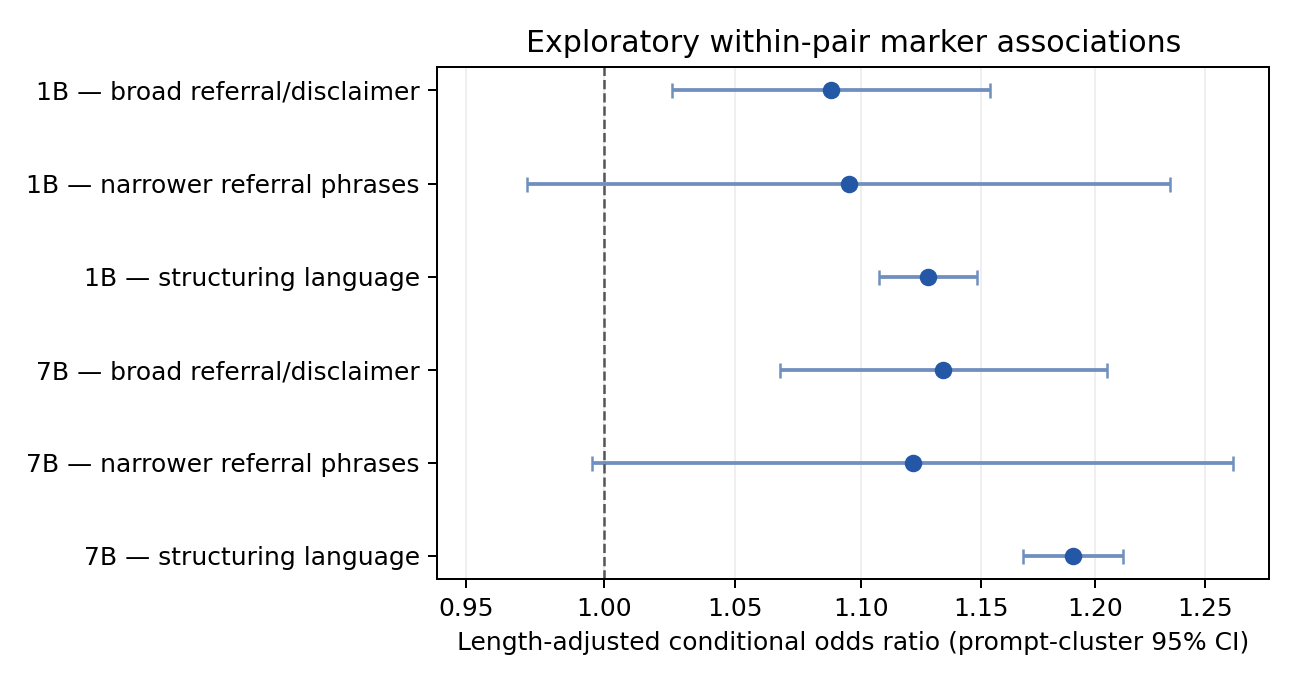
\includegraphics[width=\textwidth]{output/revision/dpo_conditional/conditional_forest.png}
\caption{Exploratory paired conditional marker associations in the 1B/7B DPO
training mixtures after flexible response-length modeling. Bars are 95\%
prompt-cluster sandwich intervals.
OR${}=1$ denotes no modeled marker--choice association, not a zero change in
preference probability.}
\label{fig:dpo-conditional}
\end{figure*}

\section{Response-cluster audit uncertainty}
\label{app:audit-bootstrap}

The 120 audit sentences come from 97 seed-0 responses. To preserve dependence
among sentences from the same response, we assign Dirichlet$(1)$ weights to
response keys in a 10{,}000-draw Bayesian bootstrap and recompute each metric.
Table~\ref{tab:audit-bootstrap} reports percentile intervals. These intervals
quantify sampling uncertainty around the AI consensus labels; they do not turn
the audit into human validation.

\begin{table}[t]
\centering
\footnotesize
\setlength{\tabcolsep}{2pt}
\begin{tabular}{lccc}
\toprule
Category & Precision 95\% & Recall 95\% & F1 95\% \\
\midrule
empathy expression & [.04,.46] & [.10,.90] & [.05,.57] \\
validation         & [.02,.84] & [.03,.98] & [.02,.83] \\
referral           & [.00,.22] & [1.00,1.00] & [.00,.36] \\
structuring        & [.35,.63] & [.74,.96] & [.49,.74] \\
\bottomrule
\end{tabular}
\caption{Bayesian response-cluster bootstrap intervals for the 120-sentence
AI consensus audit. Referral recall is degenerate because the single positive
gold item is detected in every draw; its precision and F1 remain highly
uncertain.}
\label{tab:audit-bootstrap}
\end{table}

\section{Statistical formulas}
\label{app:formulas}

Primary inference uses two-sided prompt-clustered permutation tests on
prompt-level means (10{,}000 draws), with Monte Carlo
$p=(b+1)/(B+1)$; $p<10^{-4}$ denotes zero raw exceedances.
The distinct-phrase leave-one-out removes the most frequent 3-word phrase before
recomputing the mean seeded-marker per-million. DPO comparisons use exact McNemar
tests on chosen-only versus rejected-only pairs, Haldane--Anscombe matched odds
ratios with log-scale intervals, paired risk differences with normal-approximation
intervals, and phrase occurrences per million whitespace-delimited response
words. The exploratory conditional fits use the no-intercept paired likelihood
in Section~\ref{sec:method-dpo-conditional}, a five-knot restricted cubic spline of each
side's log word count, and prompt-cluster sandwich covariance multiplied by
$G/(G-1)\,(n-1)/(n-k)$. All aggregate and length-band counts were reproduced
before fitting. A separate natural-spline implementation reproduced all six
marker coefficients within $7.6\times10^{-7}$ and their standard errors within
$3.2\times10^{-9}$. The accompanying scripts derive all statistics from the
artifact.

\end{document}
